\documentclass[journal]{IEEEtran}
\usepackage[utf8]{inputenc}
\usepackage{cite}
\usepackage{graphicx}
\usepackage{amsmath}
\usepackage{url}
\usepackage{booktabs}
\usepackage{algorithm}
\usepackage[noend]{algpseudocode}
\usepackage{hyperref}

\title{RX-INT\texttt{:} A Kernel Engine for Real-Time Detection and Analysis of In-Memory Threats}

\author{%
    \IEEEauthorblockN{Arjun Juneja \\}
    \IEEEauthorblockA{School of Electronics and Computer Science\\
    University of Southampton\\
    aj2g24@soton.ac.uk}
}

\newcommand{\code}[1]{\texttt{#1}}

\begin{document}
\maketitle

\begin{abstract}
Malware and cheat developers now leverage in-memory execution techniques to evade conventional, signature-based security products. They use methods including various types of manual mapping, module stomping, and threadless injection work entirely within the address space of a legitimate process, presenting a significant challenge for detection. Existing tools often have exploitable weaknesses, such as a dependency on user-mode PE structures or a vulnerability to time-of-check-to-time-of-use (TOCTOU) race conditions where an attacker cleans up before a periodic scan occurs. To address this, I present RX-INT, a kernel-assisted system for the detection and analysis of such threats. RX-INT employs a detection engine that combines a real-time, event-driven thread creation monitor with a stateful Virtual Address Descriptor (VAD) scanner, with various heuristics within. This stateful engine baselines both private and image-backed memory regions, using memory hashing to detect illicit modifications like module stomping. Critically, I demonstrate the practical superiority in certain benchmarks of this approach through a direct comparison with PE-sieve, a commonly used and powerful memory forensics tool. In my evaluation, RX-INT successfully detected an advanced module stomping attack and a manually mapped region that was invisible to PE-sieve. I then conclude that my hybrid, event-triggered architecture represents a tangible difference in the detection of fileless threats, with direct applications in the fields of anti-cheat and endpoint security.
\end{abstract}

\begin{IEEEkeywords}
Memory Forensics, Kernel, Anti-Cheat, Malware Detection, Evasion Techniques, Module Stomping, VAD, Windows Internals, Intrusion Detection.
\end{IEEEkeywords}

\section{Introduction}
\IEEEPARstart{T}{he} increasing sophistication of in-memory code execution techniques presents a problem to modern cybersecurity and anti-cheat methods. Attackers, ranging from state-sponsored actors to sophisticated or novice cheat developers, have largely migrated from traditional disk-based malware to `fileless' payloads that exist exclusively within the volatile memory of compromised, legitimate processes. By avoiding the filesystem, these threats bypass the primary scanning surface of most conventional antivirus (AV) and security products, allowing them to operate with a high degree of stealth. Techniques such as manual mapping, where a DLL is loaded without invoking the standard Windows loader, and module stomping, where the executable code of an already-loaded, trusted DLL is overwritten, are now commonplace in the toolkits of advanced attackers and cheat developers.
The core problem in detecting these threats lies in distinguishing legitimate, dynamic memory operations from malicious ones. Complex executables such games and web browsers, make extensive use of dynamic code generation techniques such as Just-In-Time (JIT) compilation, creating an environment where private, executable memory is not inherently suspicious. Existing user-mode memory forensics tools, while powerful, operate with a handicap. They must rely on user-mode Windows APIs (such as VirtualQueryEx and ReadProcessMemory) which can be hooked or manipulated by more privileged, kernel-mode rootkits. Furthermore, their heuristics often depend on finding structural artifacts like PE headers, which can be deliberately erased by the injector.
Kernel level detectors offer a higher privilege to monitor processes, but they are not without their own weaknesses. A reasonable approach is to periodically scan a process's memory. However, this creates a critical time-of-check-to-time-of-use (TOCTOU) vulnerability. A sophisticated attacker can perform a module stomp, execute their payload, and restore the original bytes of the legitimate module in a few hundred milliseconds which is a window of opportunity that is usually far shorter than the polling interval of a periodic scanner. This allows the threat to execute repeatedly while remaining invisible to the detector.
This paper introduces RX-INT, a kernel engine designed to overcome these problems. It operates from a kernel context and employs a novel detection engine that combines two distinct methods:
\begin{enumerate}
\item A real-time, event-driven monitor that monitors thread creation to serve as an immediate tripwire for classic injections and, more importantly, as a trigger for the VAD scanner.
\item A stateful VAD scanner that creates a comprehensive baseline of a process's memory, including the content hashes of all executable image-backed (MEM\_IMAGE) sections, allowing it to detect illicit modifications. This includes any modifications made within runtime debuggers such as x64dbg.
\end{enumerate}
The synergy between these two components of RX-INT allows it to defeat timing-based evasions. A suspicious event from the thread monitor immediately triggers an out-of-band scan from the VAD scanner, closing the TOCTOU race condition. It also introduces a fully in-kernel Import Resolver that programmatically parses the Export Address Tables (EAT) of all modules loaded in the target process. When a suspicious payload is dumped, this resolver scans the raw memory for pointers and automatically enriches the forensic data with a report of all resolved API calls, accelerating the reverse engineering process. This can be used alongside a runtime debugger to resolve any imports manually in the case of erased PE headers, or to provide a more complete picture of the threat's behavior.
To validate this approach, I conducted a direct comparison against PE-sieve (v0.4.1), a complex, widely used public memory forensics tool, using a custom-built injection suite alongside some common injectors. The evaluation yielded two critical findings: RX-INT successfully detected a manually mapped DLL with its PE headers fully erased in memory, and it successfully detected a fast-acting module stomping attack. Under the same conditions, PE-sieve failed to generate any alerts for either of these advanced techniques.
The contributions via this project are therefore:
\begin{itemize}
    \item A fully in-kernel import resolver that parses Export Address Tables (EATs) to provide automated symbolic analysis of raw memory dumps.
    \item An empirical demonstration that this architecture can detect advanced, evasive in-memory threats that are not detected by other widely-used, powerful tools.
    \item The design and implementation of a hybrid, event-triggered kernel detection architecture that is comparitively resilient to TOCTOU attacks.
\end{itemize}

\section{Background and Threat Model}
\label{sec:background}
The efficacy of modern security solutions is increasingly challenged by a class of threats that minimize or entirely eliminate their on-disk footprint. These `fileless' techniques are central to the threat model targeted in this paper, which focuses on an attacker who has achieved code execution on a target system and seeks to inject a payload into a legitimate process to operate stealthily with the goal to modify the legitimate process itself, or to hide malicious code within it. This section details the primary in-memory evasion techniques that RX-INT has been designed to detect, contextualized with adversary behavior.
\subsection{Adversary Goals and Assumptions}
This threat model assumes an adversary with user-level or administrative privileges on a 64-bit Windows system. The adversary's goal is to execute a malicious payload (such as a cheat engine, remote access trojan, or spyware) from within the address space of a trusted process. This is a common form of Masquerading, a sub-technique of Defense Evasion (TA0005) as mentioned by the MITRE ATTACK framework \cite{MITRE_ATTACK_DEFENSE_EVASION}. By operating within a legitimate process, the attacker inherits its trust level and bypasses simple process-based firewalls and monitoring tools. It is assumed the adversary has not yet compromised the kernel (i.e., has not loaded a malicious driver), meaning their actions are initiated from user mode, but they are designed to evade kernel-level detectors.
\subsection{In-Memory Evasion Techniques}
\subsubsection{Manual PE Mapping}
The standard procedure for loading a dynamic-link library (DLL) is the LoadLibrary API. These functions are heavily instrumented by security products. To bypass this procedure entirely, adversaries can implement their own PE loader. This process, known as manual mapping, involves parsing the PE file format, allocating a region of virtual memory in a target process with VirtualAllocEx, and manually copying the DLL's sections (.text, .data, etc.) into the allocated block. The injector is then responsible for performing the critical tasks of base relocation and resolving the Import Address Table (IAT) \cite{IredTeamModuleStomping}. A particularly effective variant of this technique involves subsequently erasing the PE headers from the image once it has been copied into memory, which can defeat scanners that rely on finding the IMAGE\_DOS\_SIGNATURE (`MZ') to identify executable modules, part of the reason why PE-Sieve fails. The resulting payload exists as a MEM\_PRIVATE memory region with no clear file backing, making it difficult to attribute. Advanced injectors enhance this by offering options to Clean Data Directories and Clear PE Headers. This removes all metadata from the in-memory PE image, turning it into a `freeform' blob of code and data that is very difficult to identify with signature-based scans.
\subsubsection{Module Stomping}
Module stomping is a more advanced and stealthy form of process injection. Instead of allocating new private memory, the attacker targets a legitimate, already-loaded DLL within the target process. As detailed by Hammond, this technique involves using VirtualProtectEx to make the legitimate module's executable .text section writable, which is a highly suspicious action \cite{Orr2019}. The attacker then overwrites a portion of the legitimate code—often the entry point of a known function—with their own malicious shellcode or a trampoline that redirects execution to a different memory region.
This technique is highly evasive for two primary reasons. First, the malicious code is executing from a MEM\_IMAGE memory region, which many security tools inherently trust more than MEM\_PRIVATE memory because it is associated with a legitimate, signed file on disk. Second, as noted by F-Secure, a sophisticated attacker can restore the original bytes of the stomped function immediately after their payload executes, defeating periodic memory scanners that check for integrity modifications \cite{Orr2019}. This creates a critical time-of-check-to-time-of-use (TOCTOU) vulnerability that RX-INT is specifically designed to close.
\subsubsection{Code Injection Primitive}
This is the fundamental method of placing and executing code. While classic methods use CreateRemoteThread, advanced injectors leverage a wide array of alternatives to bypass common API hooks:
\begin{itemize}
\item Thread Hijacking: Instead of creating a new thread (easily detectable), the injector suspends an existing thread in the target, overwrites its instruction pointer (RIP) to point to the malicious code, and then resumes it.
\item QueueUserAPC: A `threadless' injection that queues an Asynchronous Procedure Call (APC) to a legitimate thread. The malicious code is executed when the thread enters an alertable wait state, avoiding the creation of a new thread entirely.
- Kernel Callbacks \& FakeVEH: Abuses kernel callback functions or set up fake Vectored Exception Handlers (FakeVEH) to hijack the process's control flow in response to system events or deliberately triggered exceptions.
\end{itemize}
\subsubsection{Post-Injection Stealth and Obfuscation}
After the code is mapped and a thread is executed, injectors can employ a final layer of techniques to hide the thread itself from analysis tools.
\begin{itemize}
\item Cloak Thread: The thread is created with characteristics that hide it from standard user-mode debuggers.
\item Fake Start Address: The thread's start address in its control structures (TEB/PEB) is pointed to a benign location, while the actual execution begins elsewhere. This is intended to fool scanners that only check the `official' start address.
\item Skip Thread Attach: Manipulates thread flags to prevent standard DLL\_THREAD\_ATTACH notifications from being sent to the process's loaded modules.
\end{itemize}
\subsection{Kernel-Level Threats and Detection Challenges}
While our threat model focuses on user-mode injection, the design of a detector such as this must be informed by the challenges of kernel-level security. The `OnThreadNotify' callback, operating at the kernel level, is designed to catch the creation of threads regardless of user-mode `cloaking' or `fake start address' tricks, providing a robust, low-level view of process execution that is difficult for a user-mode attacker to subvert. The Windows kernel's internal memory management is organized by a tree of Virtual Address Descriptor (VAD) structures, which are opaque to user-mode code \cite{Russinovich2022}. Kernel-mode detectors can traverse this tree to build a complete and accurate map of a process's memory layout. However, as recent surveys on kernel-level rootkits have shown, even kernel components can be attacked, and relying on a single detection methodology is often insufficient \cite{nadim2023kernellevelrootkitdetectionprevention}. Therefore, a modern detector must employ a multi-layered approach to be effective against an informed adversary. RX-INT was designed with this principle in mind, combining real-time event monitoring with stateful memory analysis to provide defense. 

\section{System Design and Architecture}
\label{sec:design}
To address the complex threat model of in-memory attacks, RX-INT is designed as a modular, client-server system that separates the user-facing control logic from the privileged kernel-mode detection engine. This architecture, shown in Fig. \ref{fig_architecture}, allows for a clean separation of concerns and provides a flexible framework for real-time monitoring and analysis. The system is comprised of a user-mode client, a kernel-mode driver, and a well-defined IOCTL interface that facilitates their communication.
\begin{figure}[!t]
\centering
% This is where you will place your architecture diagram.
% Create a simple diagram showing:
% [TUI Client] <--> [IOCTL Interface] <--> [Kernel Driver]
% And within the driver, show the Detector class containing the
% Thread Monitor, VAD Scanner, and Export Resolver.
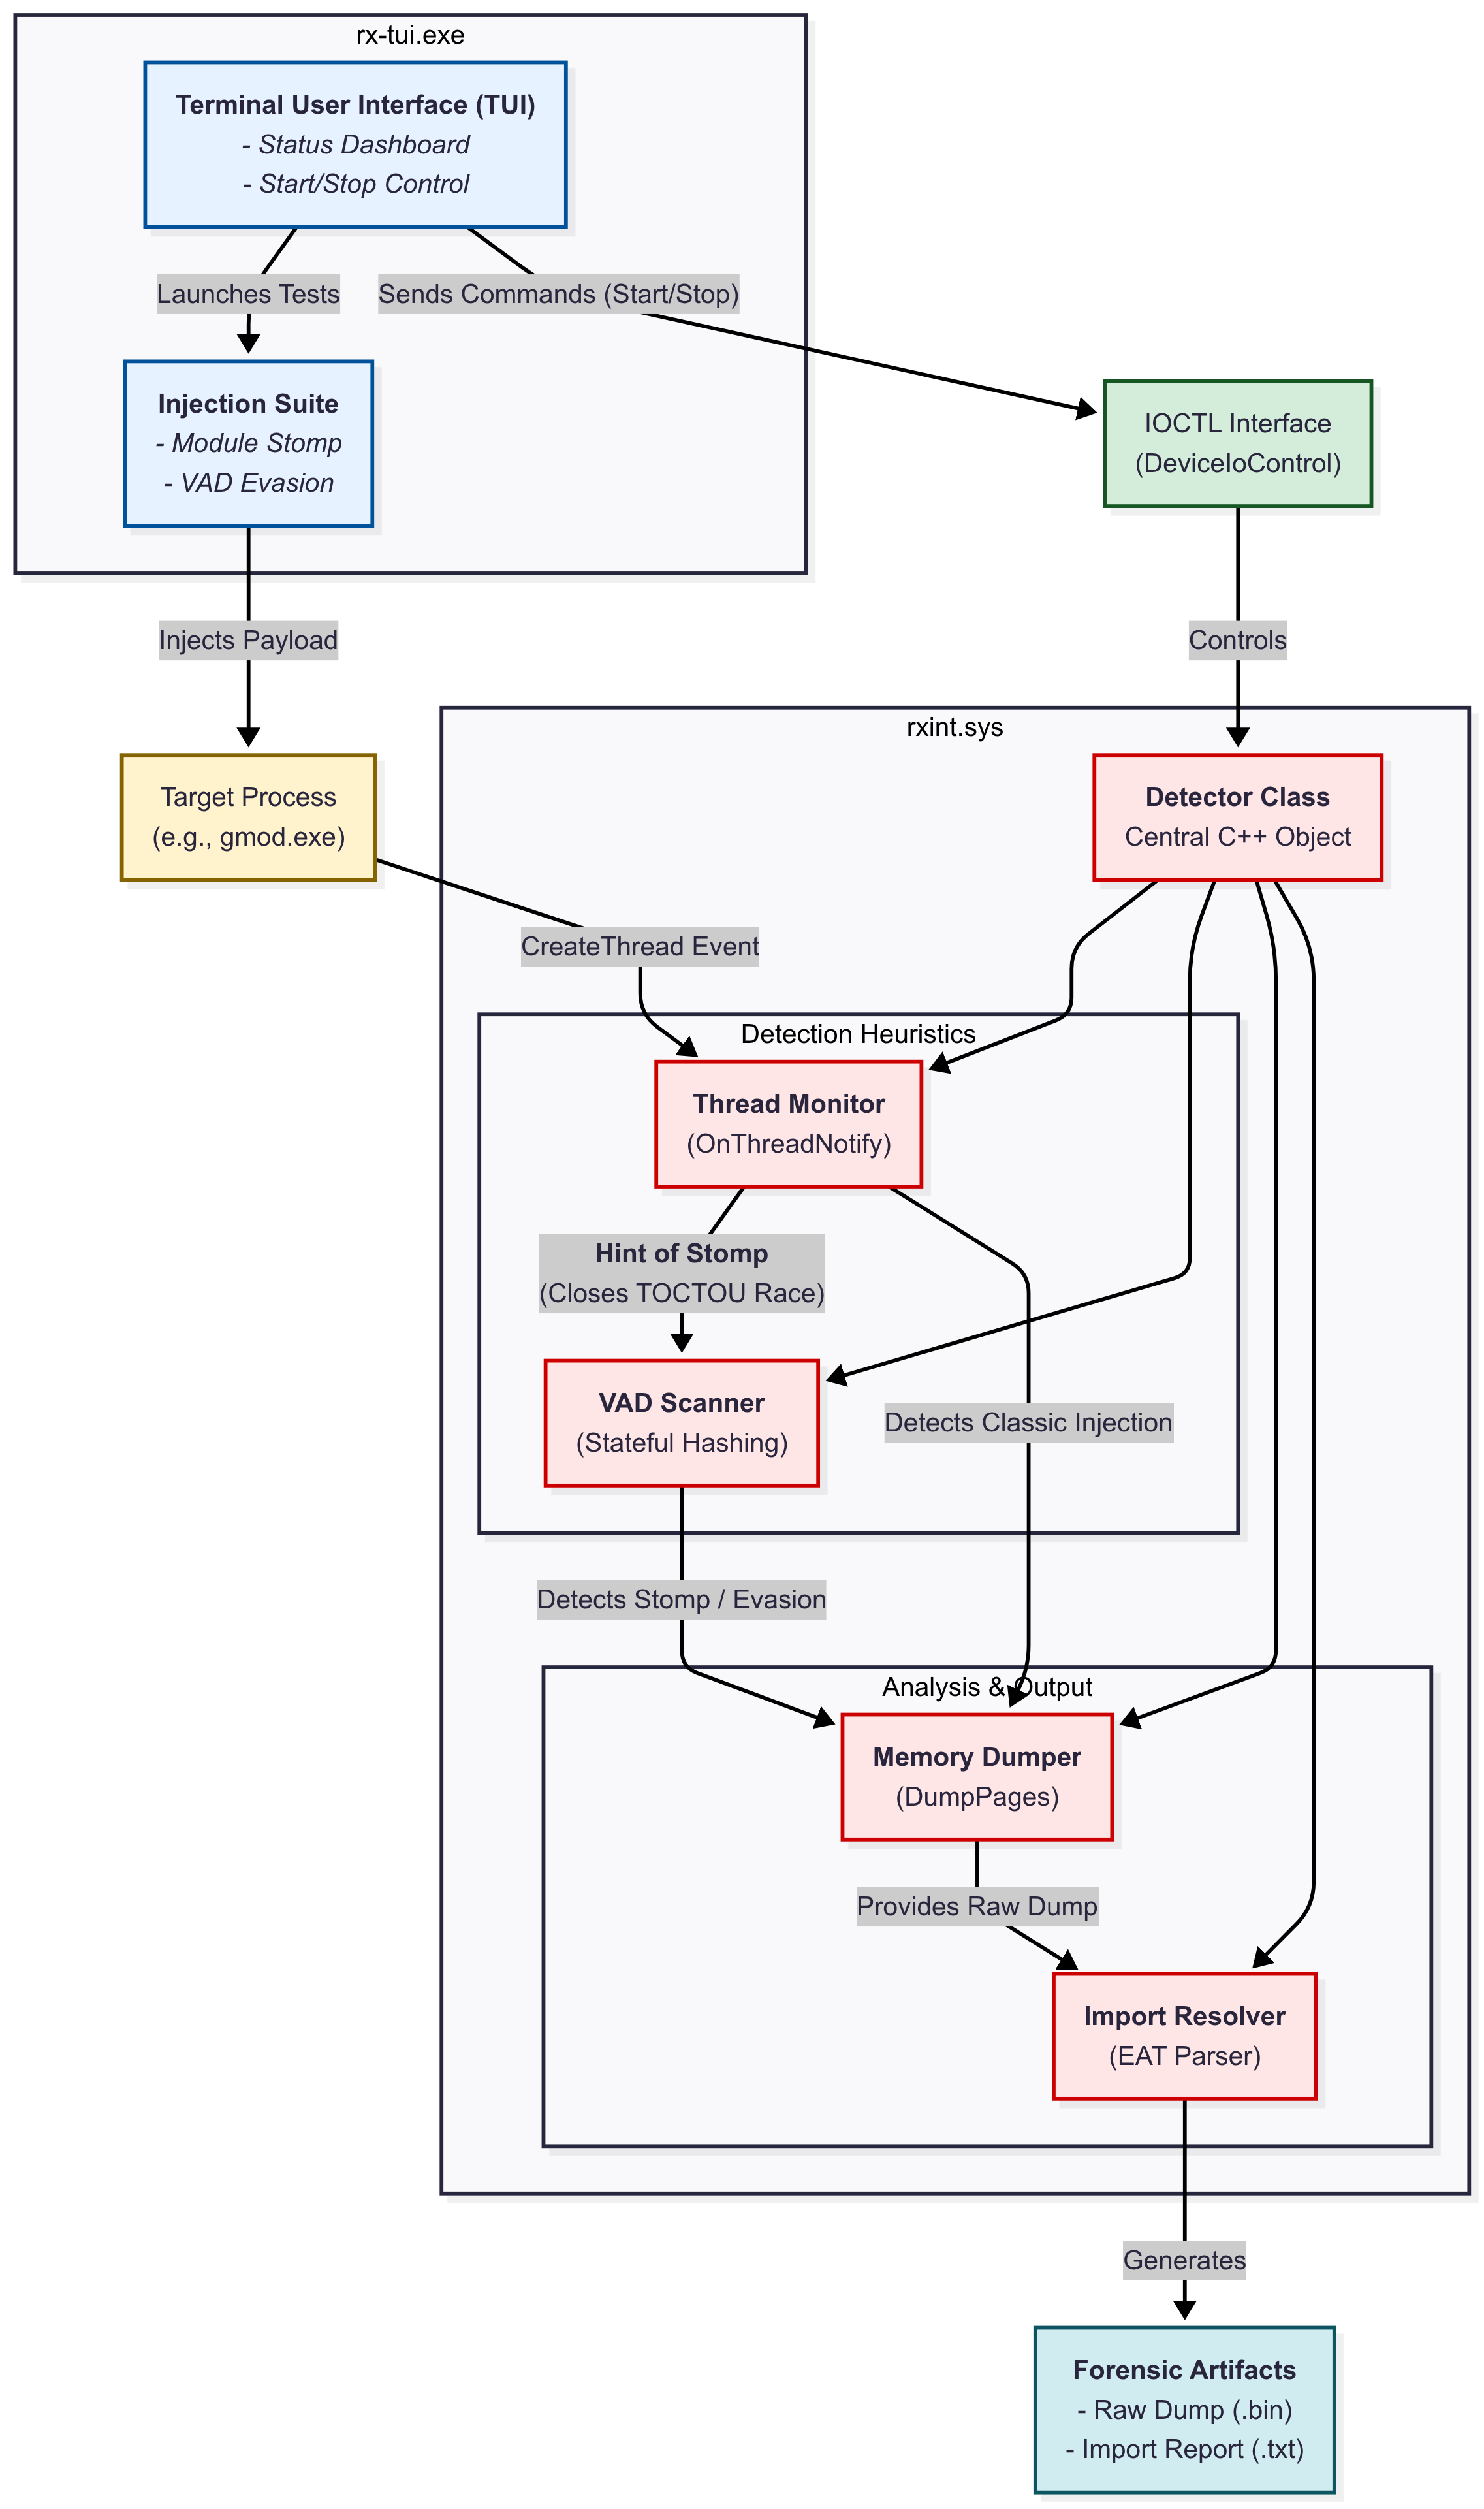
\includegraphics[width=0.9\columnwidth]{figures/architecture.png}
\caption{High-level architecture of the RX-INT system, showing the interaction between the user-mode client and the kernel-mode driver components.}
\label{fig_architecture}
\end{figure}
\subsection{User-Mode Client (\texttt{rx-tui.exe})}
The primary interface for an analyst is the RX-INT Terminal User Interface (TUI). This component is a standalone C++23 executable with zero external dependencies, utilizing a custom, double-buffered rendering engine built on the native Windows Console API for a responsive, flicker-free experience. The TUI's responsibilities are threefold:
\begin{itemize}
\item \textbf{Control:} It provides the operator with commands to start and stop monitoring on any target process, which is specified by its Process ID (PID). This explicit, user-driven control model is crucial for avoiding the false positives that can arise from attaching to a process during its noisy initialization phase.
\item \textbf{Status Monitoring:} The TUI provides a persistent dashboard that displays the real-time status of the kernel driver (e.g., Idle, Monitoring), the PID of the currently monitored process, and key performance metrics such as the driver's paged and non-paged kernel pool memory footprint.
\item \textbf{Evaluation:} The client contains an integrated "Injection Suite" that allows the operator to launch a curated set of advanced, in-memory attacks against a target process. This serves as a built-in validation and evaluation harness for the kernel driver's detection capabilities.
\end{itemize}
\subsection{IOCTL Interface}
Communication between the user-mode client and the kernel driver is facilitated through a standard, synchronous Windows I/O model. Upon loading, the driver creates a named device object (\\Device\\RxInt) and a corresponding symbolic link (\\??\\RxInt) that is visible to user-mode applications. The TUI client uses the CreateFile API to open a handle to this device, and all subsequent commands are sent via DeviceIoControl calls.
This interface is defined by a shared header (ioctl.h) containing a set of custom I/O Control Codes (IOCTLs). The primary IOCTLs allow the client to pass a RXINT_MONITOR_INFO structure, containing the target PID and a custom dump path format, to begin a monitoring session, and to send a command to stop the session. Additional IOCTLs are used to query the driver for its current status and memory usage statistics, enabling the TUI's live dashboard.
\subsection{Kernel Driver (\texttt{rxint.sys})}
The core of the system is a C++ kernel-mode driver that performs all detection and analysis. The driver is architected around a central Detector class, which encapsulates all state and logic. To ensure stability and prevent resource leaks in the hostile kernel environment, the driver makes extensive use of modern C++ RAII (Resource Acquisition Is Initialization) principles. Custom wrapper classes (ProcessReference, SpinLockGuard) provide safe, automatic management of kernel resources such as PEPROCESS object references and KSPIN_LOCKs. The driver's detection capabilities are divided into two primary, synergistic subsystems: an event-driven thread monitor and a stateful VAD scanner. Upon a successful detection, the driver is responsible for dumping the suspicious memory region and its automatically generated import analysis report to disk.


\bibliographystyle{IEEEtran}
\bibliography{IEEEabrv,references}

\end{document}